\chapter{Directorio del documento}
La plantilla y el perfil de TeXstudio con el que se ha elaborado esta plantilla están configurados de forma que el directorio en el que se localiza el archivo \textit{raiz.tex} debe contener una carpeta de nombre <<compilacion>> en la que se generan los archivos tras la compilación, incluido el .pdf resultado.

Para la organización del resto de archivos, se emplean las carpetas que se muestran en la figura \ref{subfig:directorio-raiz}.

Las partes y capítulos se pueden organizar en subcarpetas dentro de <<\textit{cuerpo}>>; para organizar los .tex y archivos a incluir en cada capítulo, la plantilla ofrece las sub-subcarpetas mostradas en la  figura \ref{subfig:directorio-cap}.

La estructura completa del directorio es la mostrada en la figura \ref{fig:directorio-raiz-completo}.
%
\begin{figure}
	\centering
	\begin{subfigure}[b]{1\textwidth}
		\centering
		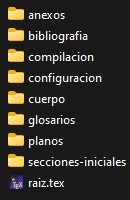
\includegraphics[scale=1]{cuerpo/cap-directorio/imagenes/directorio-raiz}
		\caption[Directorio raíz.]{Directorio raíz. Carpetas que contiene el directorio raíz del archivo \textit{raiz.tex}, que conforma el archivo .tex raíz del documento.}
		\label{subfig:directorio-raiz}
	\end{subfigure}
%	\vfill
	\begin{subfigure}[b]{1\textwidth}
		\centering
		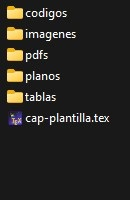
\includegraphics[scale=1]{cuerpo/cap-directorio/imagenes/sub.directorio}
		\caption[Sub-directorio para capítulo.]{Sub-directorio para capítulo. Carpetas para organizar los archivos correspondientes.}
		\label{subfig:directorio-cap}
	\end{subfigure}
	\caption{Estructura del directorio de la plantilla.}
	\label{fig:directorios}
\end{figure}
%
\begin{figure}[h]
	\centering
	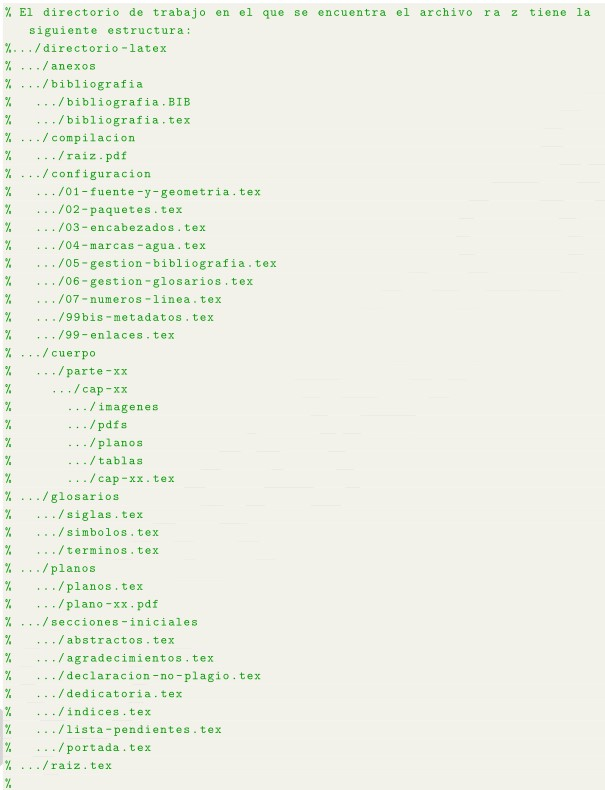
\includegraphics[scale=1, frame]{cuerpo/cap-directorio/imagenes/directorio-raiz-completo}
	\caption[Directorio raíz completo.]{Directorio raíz completo.}
	\label{fig:directorio-raiz-completo}
\end{figure}